\documentclass{article}
\usepackage{amsmath}
\usepackage{hyperref}
\usepackage{tikz}
\usetikzlibrary{shapes}
\begin{document}

\title{Folded Balun}
\maketitle

This document has been written as my attempt to understand the operation of a Folded Balun, also known as a Pawsey Stub.  I used information drawn from \cite{stack_exchange}\cite{antenna_theory}\cite{duffey}.  It is the work of an amateur in this field, rather than an expert.

\begin{figure}[h]
\caption{400 MHz UHF Dipole with a folded balun. The feedline and stub are constructed from rigid coax.}
\label{fig:uhf_diople}
\begin{center}
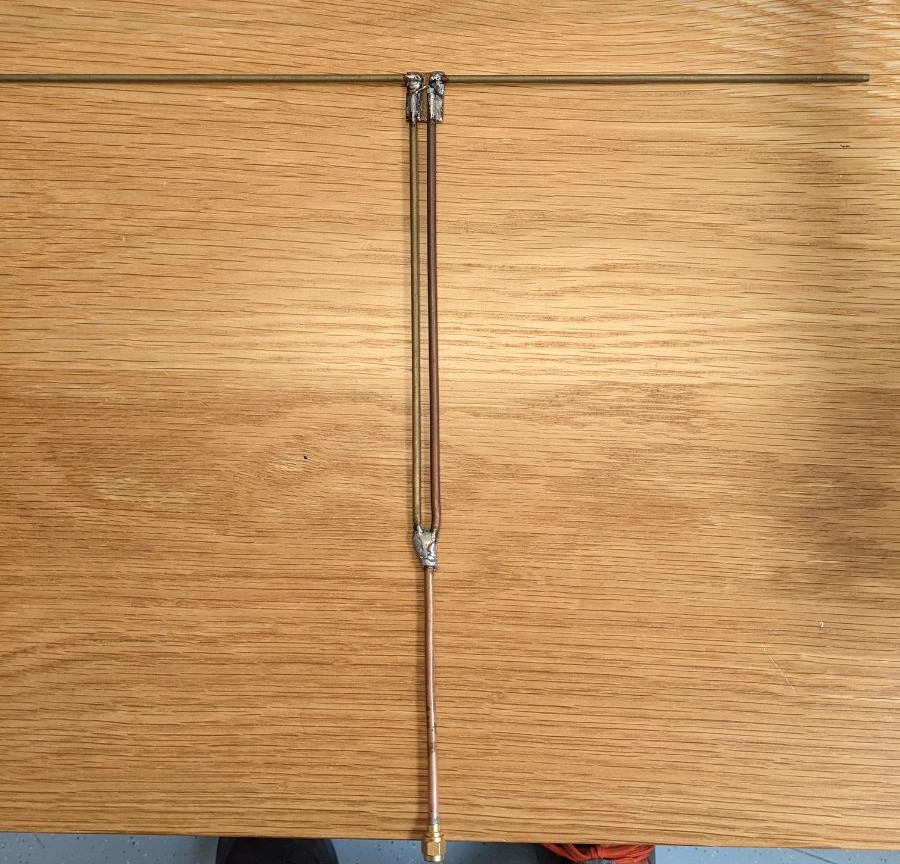
\includegraphics{uhf_dipole.jpg}
\end{center}
\end{figure}

\begin{figure}[h]

\caption{Dipole with coax feedline and stub.  Only the shield of the stub is connected.}
\label{fig:assembly}
\vspace{5mm}
\centering
\begin{tikzpicture}
\node (A) at (2,1) [cylinder, shape border rotate=90, draw, minimum height=4cm, minimum width=1cm] {};
\node[] at (2,1) {Stub};
\node (B) at (3.5,0) [cylinder, shape border rotate=90, draw, minimum height=6cm, minimum width=1cm] {};
\node[] at (3.5,1) {Coax};

% right diople arm
\draw (4.0,3) -- (4.0,3.5);
\draw (4.0,3.5) -- (9.0,3.5);

% left diople arm
\draw (3.5,3) -- (3.5,3.5);
\draw (3.5,3.5) -- (-1.5,3.5);

% stub connections
\draw (2.5,3) -- (2.5,3.5);
\draw (2.5,-0.75) -- (3,-0.75);

% unused stub centre
\draw (2,3) -- (2,3.35);
\draw (2,-0.9) -- (2,-1.2);

\node[] at (3.75,4) {Feedpoint};

\end{tikzpicture}
\end{figure}

Consider a dipole driven by a coax feedline.  The purpose of the balun is to remove any current on the coax shield outer, to ensure the currents in each dipole arm are balanced.

The balun is formed by the addition of a quarter wave stub to an existing coax feedline and dipole assembly.  The stub should be constructed from the same coax as the feedline, so that it's RF properties are similar.  The balun is formed by the interaction of the stub with the existing coax feedline and dipole.

Only the shield of the stub is used.  The inner of the coax feedline is connected to the stub at the feedpoint, and the stub is connected to the feedline coax shield a quarter wavelength from the feedpoint.

\begin{figure}[h]
\caption{Dipole in parallel with shorted twin-wire transmission line formed by the coax and stub shield.}
\label{fig:shorted}
\vspace{5mm}
\centering
\begin{tikzpicture}
\node (A) at (3,1) [cylinder, shape border rotate=90, draw, minimum height=4cm, minimum width=1cm] {};
\node (B) at (4.5,1) [cylinder, shape border rotate=90, draw, minimum height=4cm, minimum width=1cm] {};

% right diople arm
\draw (4.0,1) -- (4.0,3.5);
\draw (4.0,3.5) -- (9.0,3.5);

% left diople arm
\draw (3.5,3.5) -- (-1.5,3.5);

% stub connections
\draw (3.5,3) -- (3.5,3.5);
\draw (3.5,-0.75) -- (4,-0.75);

\node[] at (3.75,4) {Feedpoint};

\end{tikzpicture}
\end{figure}

Consider just the coax shield outer and the stub in Figure \ref{fig:shorted}.  We can see two similar conductors with a constant separation, shorted at one end.  It can be viewed a twin wire transmission line, one quarter wavelength long, connected across the feedpoint.  The short is transformed to a high impedance across the feedpoint. Thus the addition of the stub has no affect on the dipole operation when fed by balanced currents.

\begin{figure}[h]
\caption{Folded balun currents.  The impedance $Z$ of the coax shield outer and stub are similar, so the currents $I_{outer}$ and $I_{stub}$ are the same magnitude but opposite sign.}
\label{fig:currents}
\vspace{5mm}
\centering
\begin{tikzpicture}

\node[] at (4.25,4) {Feedpoint};

% right diople arm, connected to shield
\draw (6.0,1) -- (6.0,3.5); % outer
\draw (5.0,1) -- (5.0,3.5); % inner
\draw (5.0,3.5) -- (9.0,3.5); % diople arm

% left dipole arm, connected to coax inner & stub
\draw (3.5,1) -- (3.5,3.5);    % coax inner 
\draw (2.5,1) -- (2.5,3.5);    % stub
\draw (3.5,3.5) -- (-0.5,3.5); % diople arm

\node[] at (2.5,0.75) {Stub};
\node[] at (3.5,0.75) {Coax};
\node[] at (3.5,0.4) {Inner};
\node[] at (5.5,0.75) {Shield};

\node[] at (4.75,2) {$I$};
\node[] at (3.75,2) {$-I$};
\node[] at (6.5,2) {$I_{outer}$};
\node[] at (2,2) {$I_{stub}$};

\end{tikzpicture}
\end{figure}

In practice some of the differential, balanced current flowing inside the coax feedline is converted to common mode current.  Consider current on the coax shield inner $I$ at the feedpoint (Figure \ref{fig:currents}).  It will be split between the desired dipole arm and the coax shield outer. The amount of current flowing down the coax shield outer $I_{outer}$ depends on the impedance $Z$ of this path.

The current flowing in the coax inner $-I$ is equal in magnitude but opposite it direction to the current on the coax shield inner.  This current will be split in the same way, the desired current along the dipole arm, and the undesired component $I_{stub}$ down the stub.  Because the stub is made of the same material as the feedline, and is located at approximately the same position, $Z$ will be the same, and the current flowing will be the same magnitude but opposite sign $I_{stub}=-I_{outer}$.  

These currents cancel at the point where the stub connects to the coax shield, resulting in zero current on the coax shield outer beneath this point - achieving the goal of the balun.

Now the coax shield outer and stub are carrying common mode RF currents and are a significant fraction of a wavelength. However the stub and coax shield outer currents are equal and opposite, the conductors are close together, so the far field radiation is cancelled.  In other words, they form a transmission line.  A transmission line, by definition, does not radiate RF power. This means that no RF power is radiated from the common mode currents on the coax shield outer or stub, and hence all RF power must be radiated by the dipole.

In short, the stub draws a current from the coax inner that cancels the current flowing down the outside of the coax shield \cite{antenna_theory}.

Owen Duffey \cite{duffey} has simulated this balun with asymmetric loads (e.g. offset fed dipoles, or a real-world HF antenna with random objects in the near field) and has concluded it is only useful for highly symmetric loads (e.g. a UHF dipole, where the short wavelength makes it easy to have no objects in the near field).  This is consistent with the explanation above, as it's operation depends on the currents in both dipole arms being equal and opposite.

\bibliographystyle{plain}
\bibliography{folded_balun_refs}
\end{document}
